\chapter{Annexes}

\section{Annexe A : Schémas résumant le projet dans chacun de ses modes de fonctionnement}

\subsection{Mode apprentissage}

Dans le mode apprentissage, le logiciel doit permettre à l’utilisateur de rentrer dans la
base de données des documents manuscrits avec une vérité terrain ou non. Dans le second cas,
l’utilisateur rentre à la main une transcription à partir de l’IHM. La base ainsi créée est
utilisée pour permettre un apprentissage du reconnaisseur.

\paragraph{}
\begin{mdframed}[frametitle={Annexe A.1.1 : Avec détection de lignes}, innerbottommargin=10]
\begin{center}
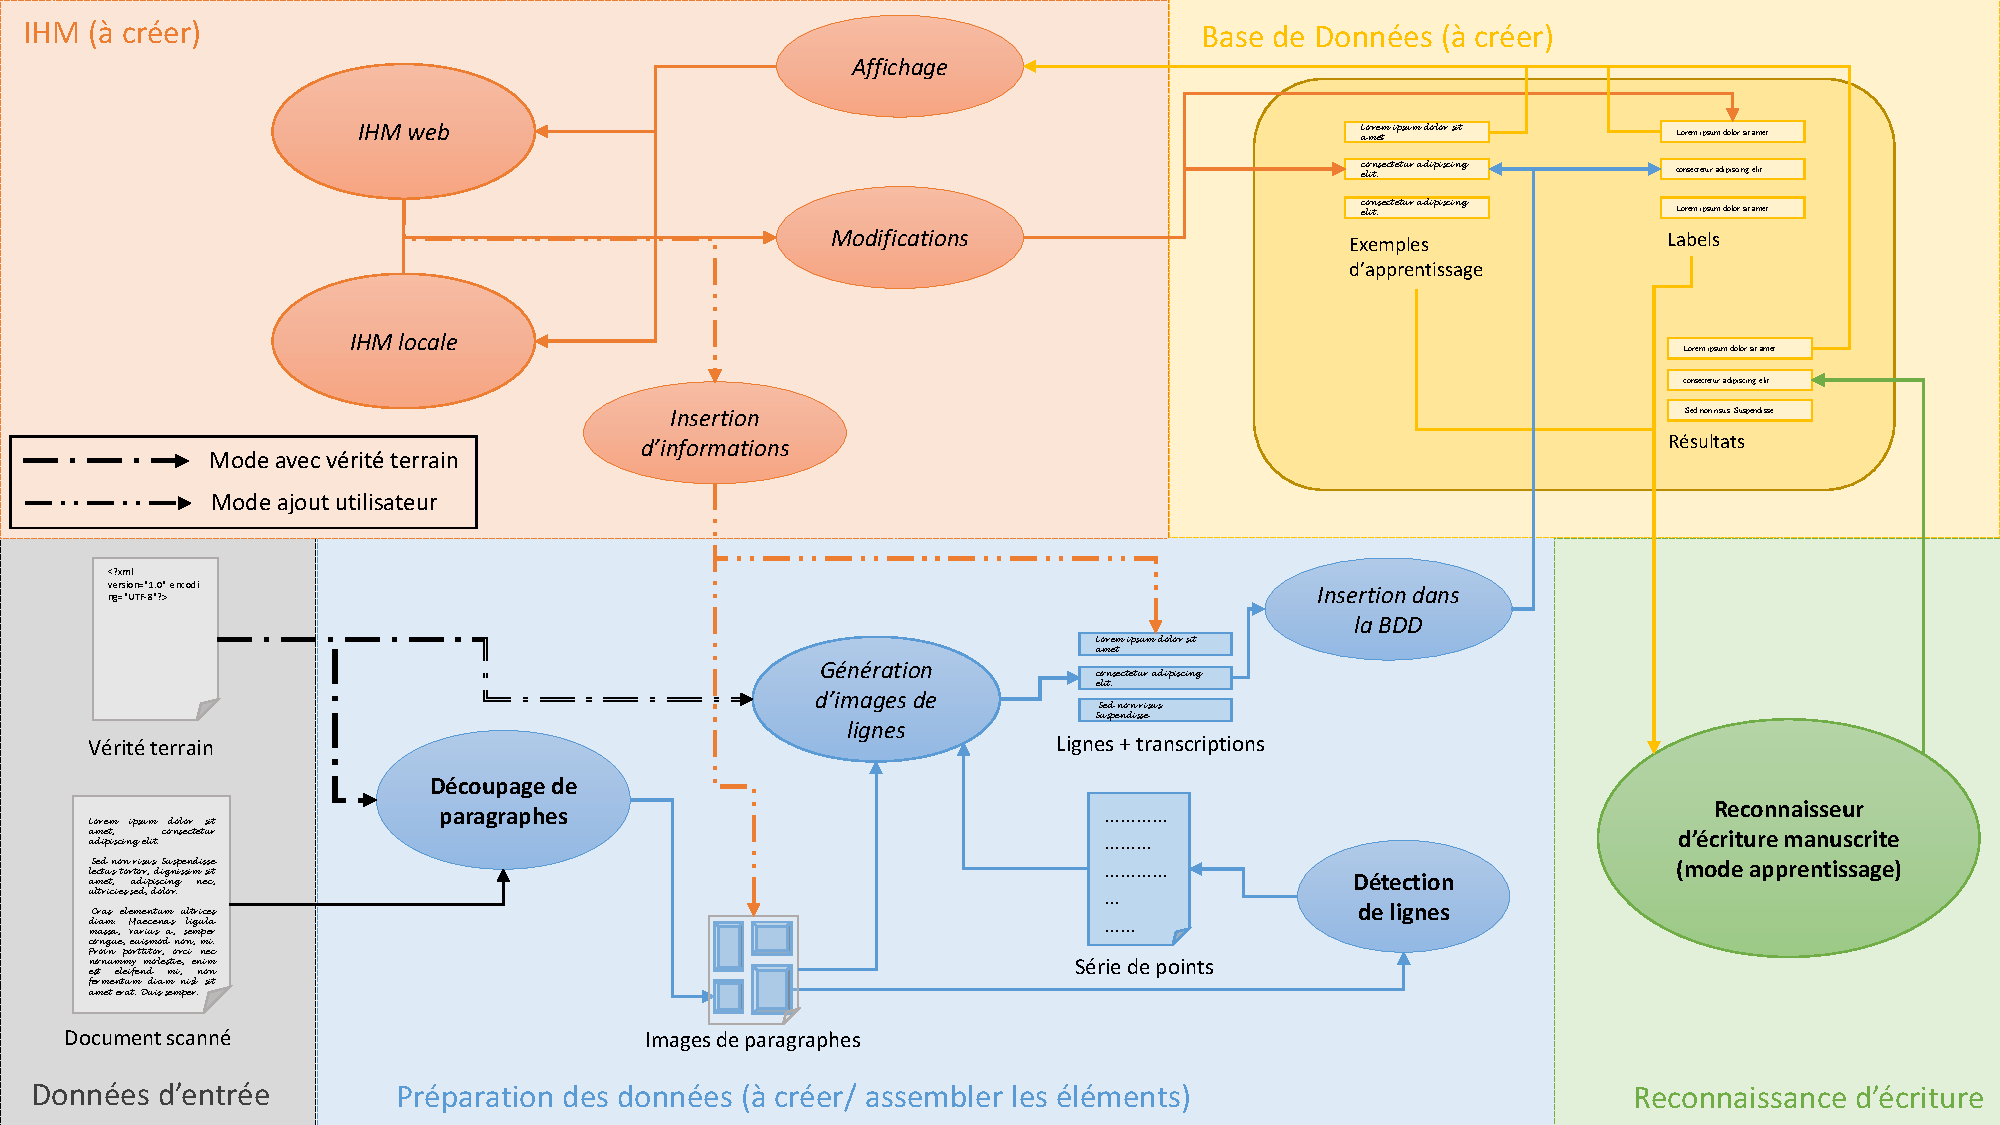
\includegraphics[width=\linewidth]{schema_mode1.1.pdf}
\end{center}
\end{mdframed}

\newpage

\paragraph{}
\begin{mdframed}[frametitle={Annexe A.1.2 : Sans détection de lignes}, innerbottommargin=10]
\begin{center}
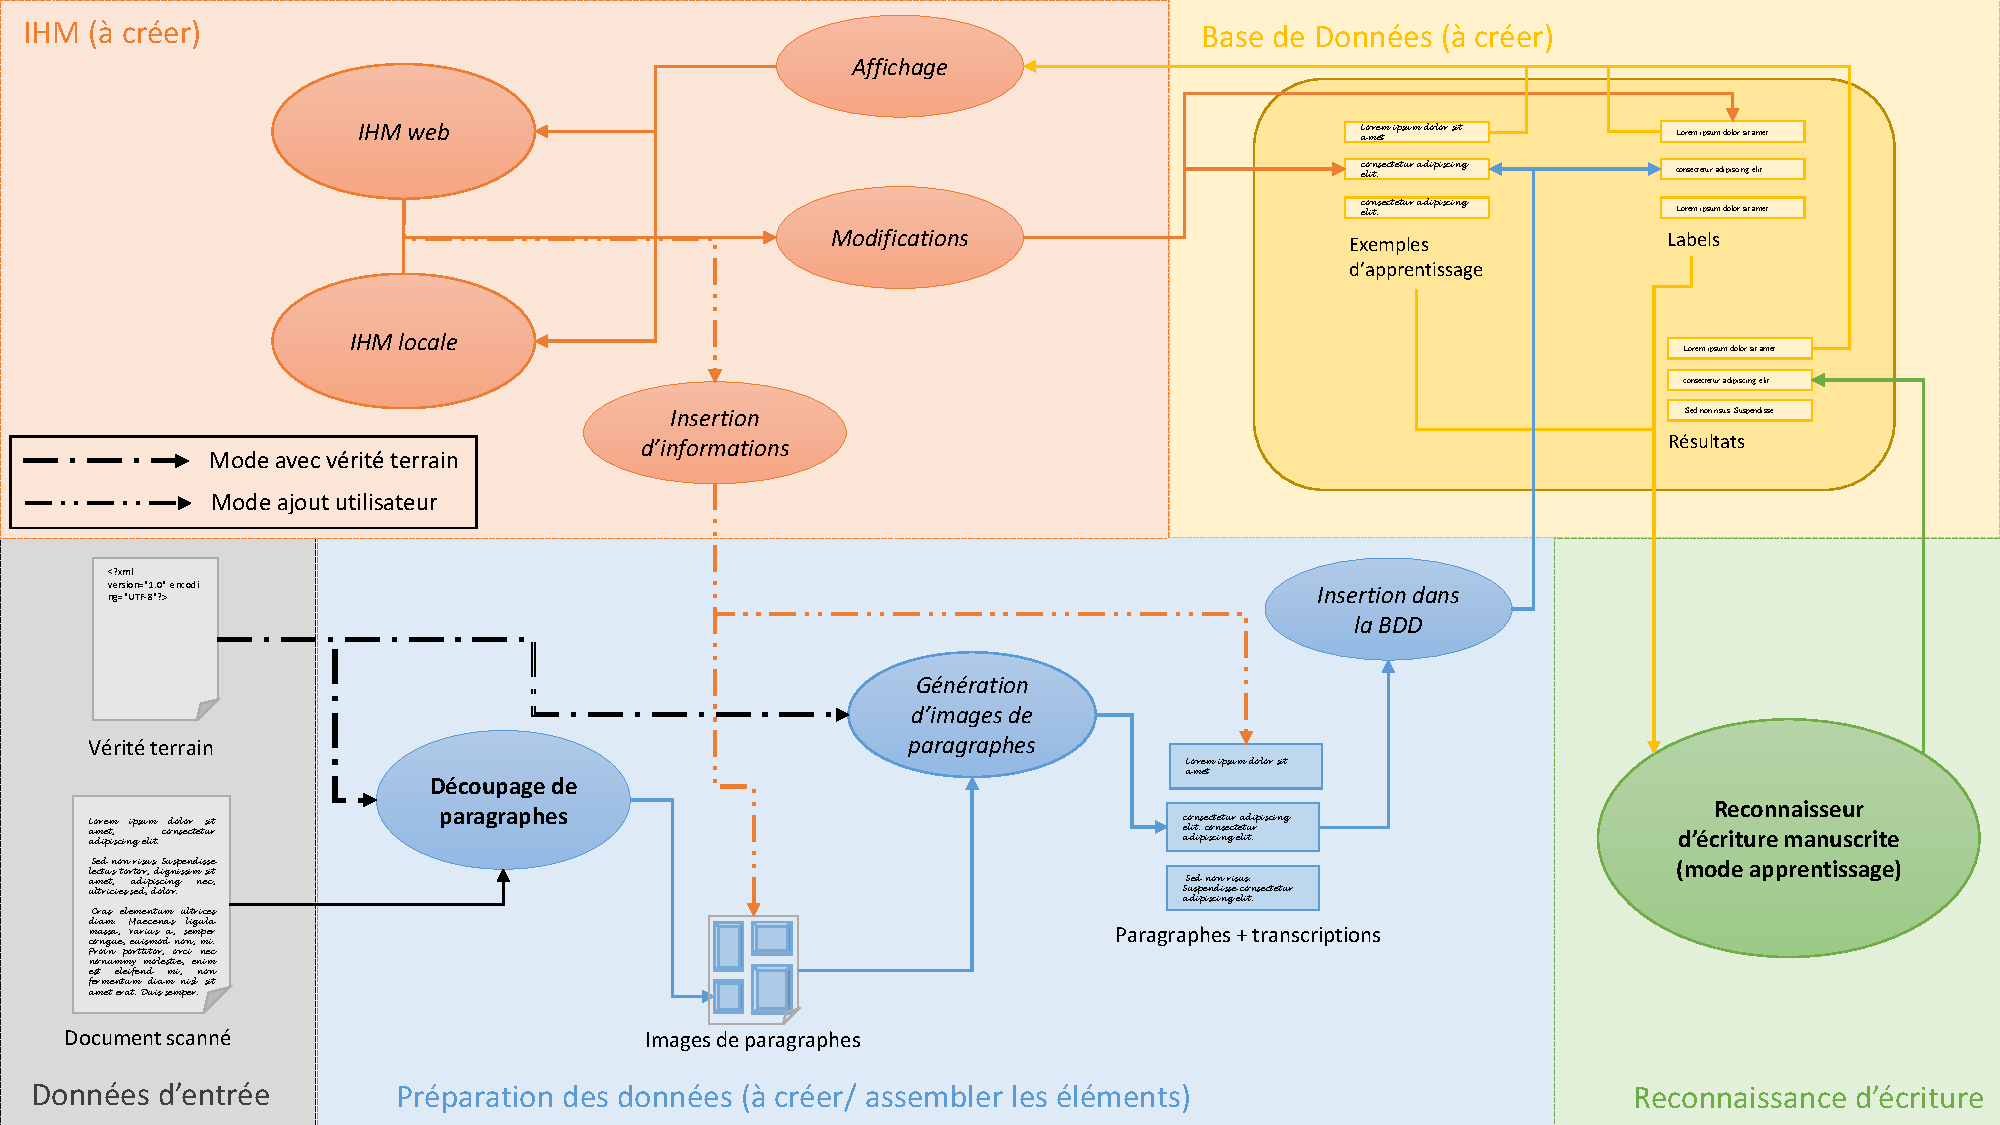
\includegraphics[width=\linewidth]{schema_mode1.2.pdf}
\end{center}
\end{mdframed}

\subsection{Mode évaluation}

Dans le mode évaluation, le logiciel doit permettre à l’utilisateur de rentrer des documents
dans la base de données avec une vérité terrain. La base créée est utilisée pour évaluer
le reconnaisseur et vérifier son efficacité.

\paragraph{}
\begin{mdframed}[frametitle={Annexe A.2.1 : Avec détection de lignes}, innerbottommargin=10]
\begin{center}
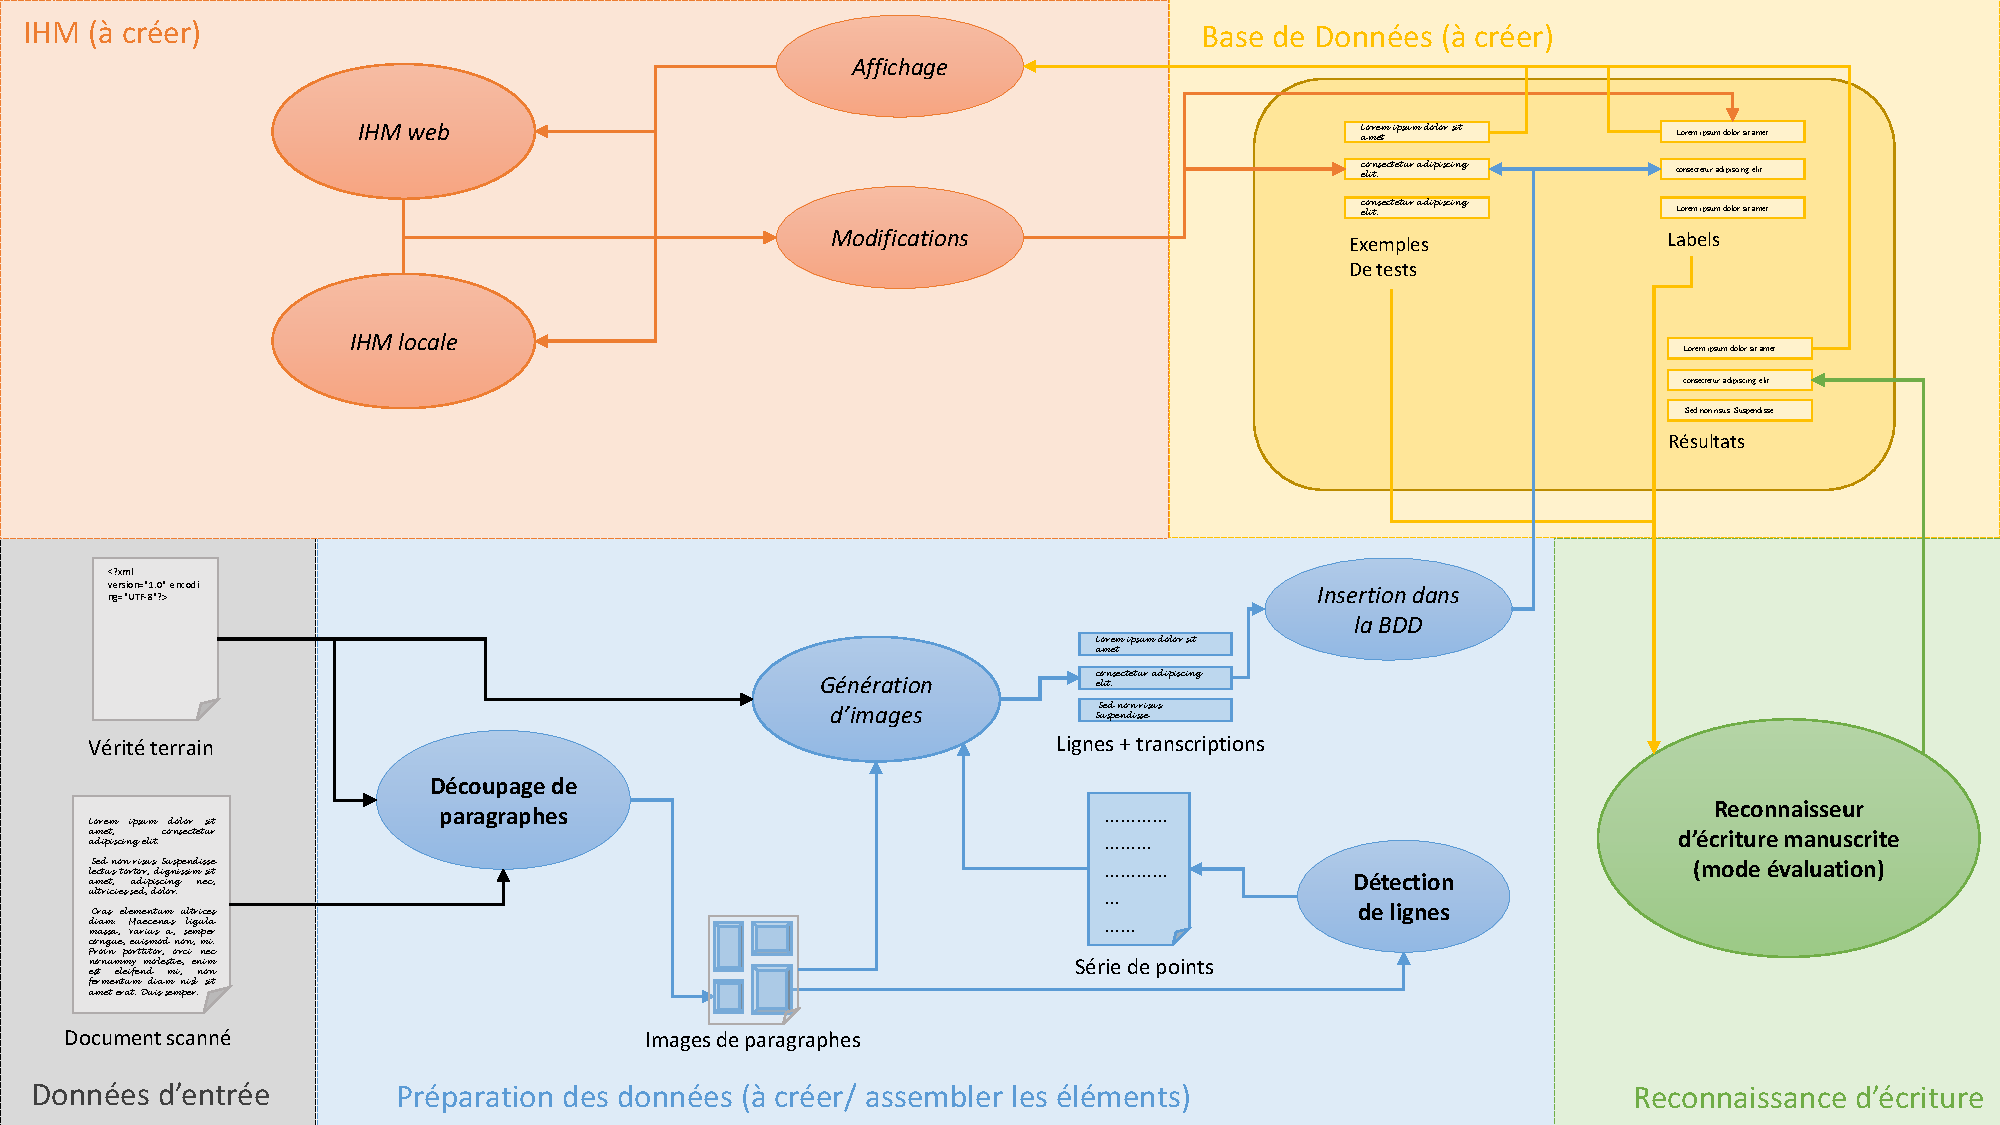
\includegraphics[width=\linewidth]{schema_mode2.1.pdf}
\end{center}
\end{mdframed}

\paragraph{}
\begin{mdframed}[frametitle={Annexe A.2.2 : Sans détection de lignes}, innerbottommargin=10]
\begin{center}
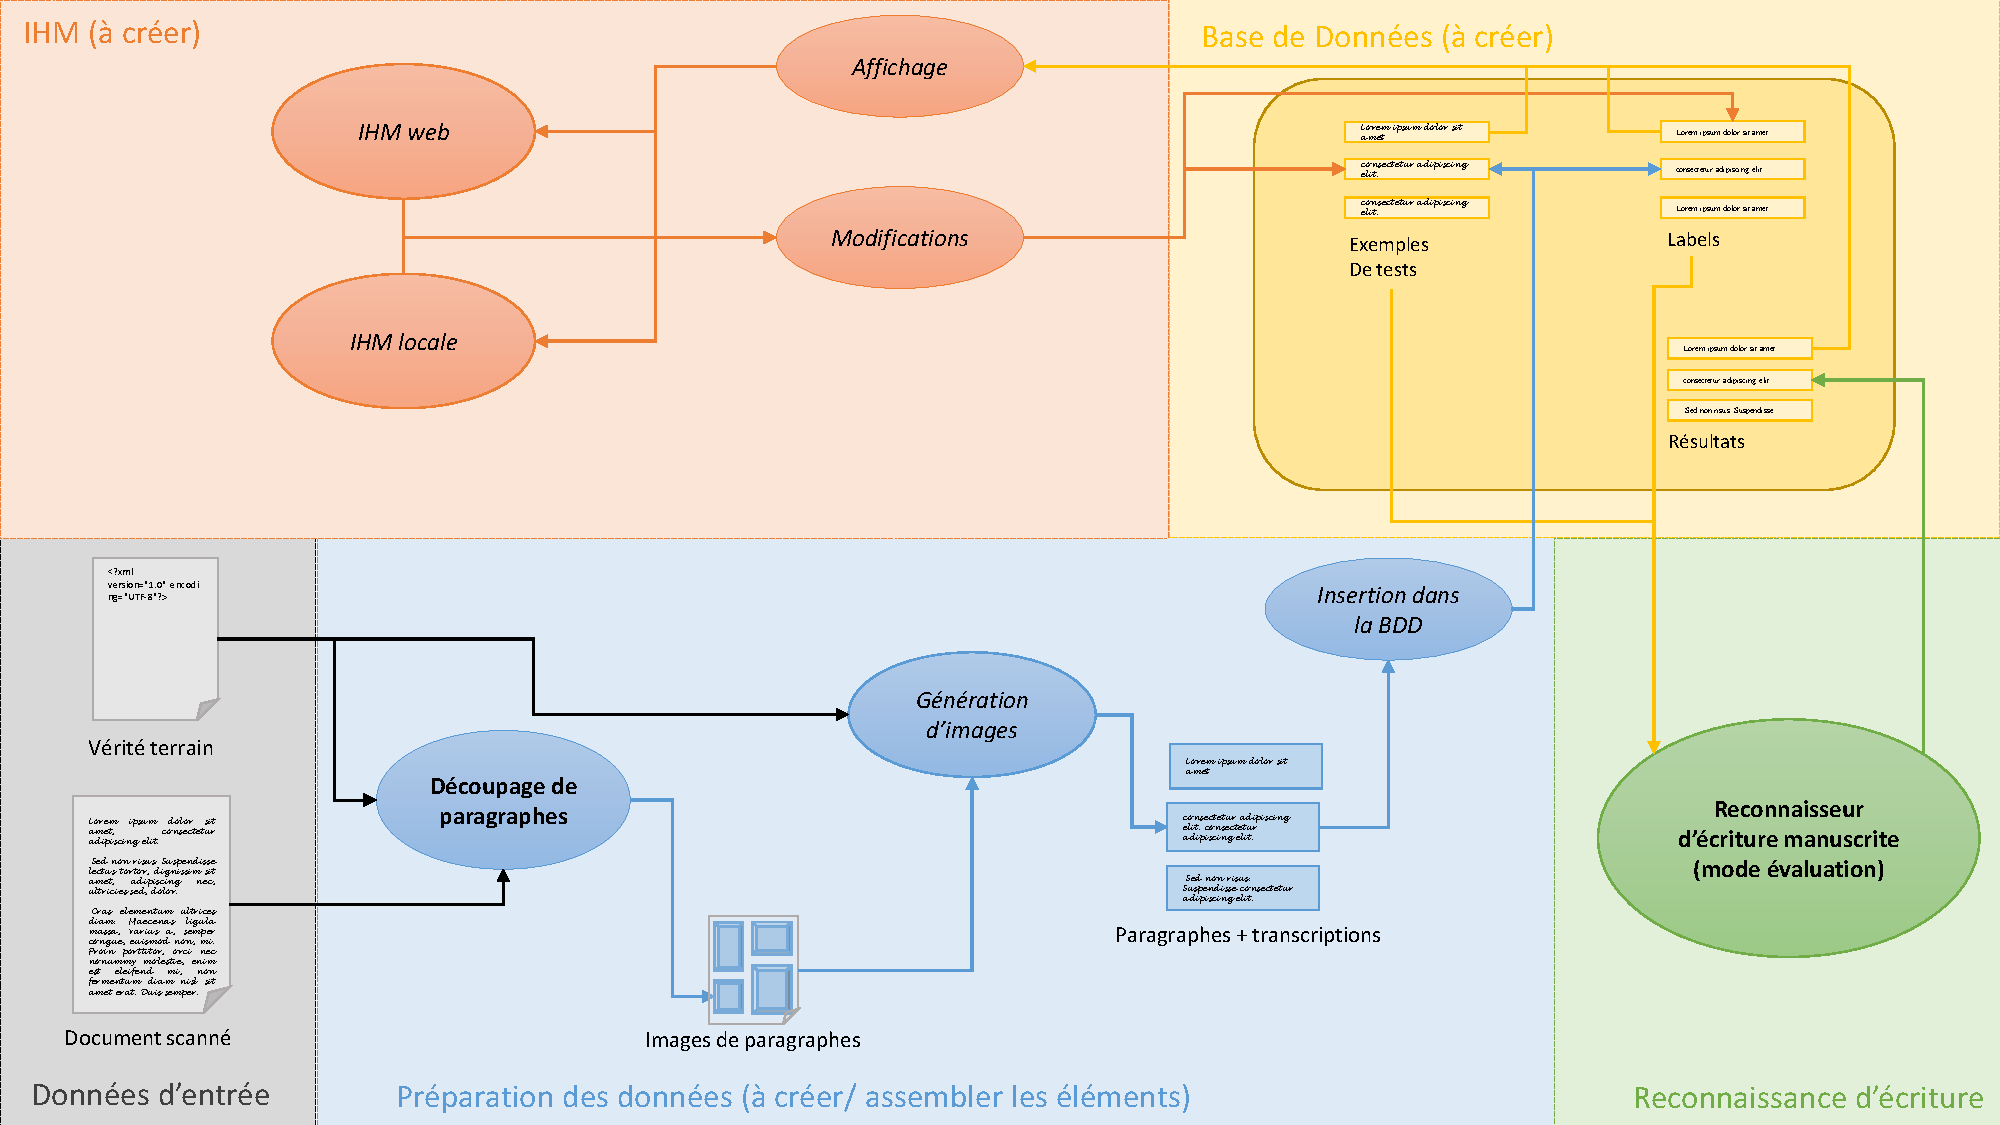
\includegraphics[width=\linewidth]{schema_mode2.2.pdf}
\end{center}
\end{mdframed}

\subsection{Mode production}

Dans le mode production, le logiciel doit permettre à l’utilisateur de rentrer des documents
sans vérité terrain ni transcription. Le reconnaisseur fournit alors une retranscription du
document. Ce mode peut être utilisé pour plusieurs cas d’utilisation : la transcription fournie
par le reconnaisseur est complétée par l’utilisateur et permet de transcrire rapidement un document
numériquement. Il peut aussi être utilisé pour effectuer des démonstrations.

\newpage

\paragraph{}
\begin{mdframed}[frametitle={Annexe A.3.1 : Avec détection de lignes}, innerbottommargin=10]
\begin{center}
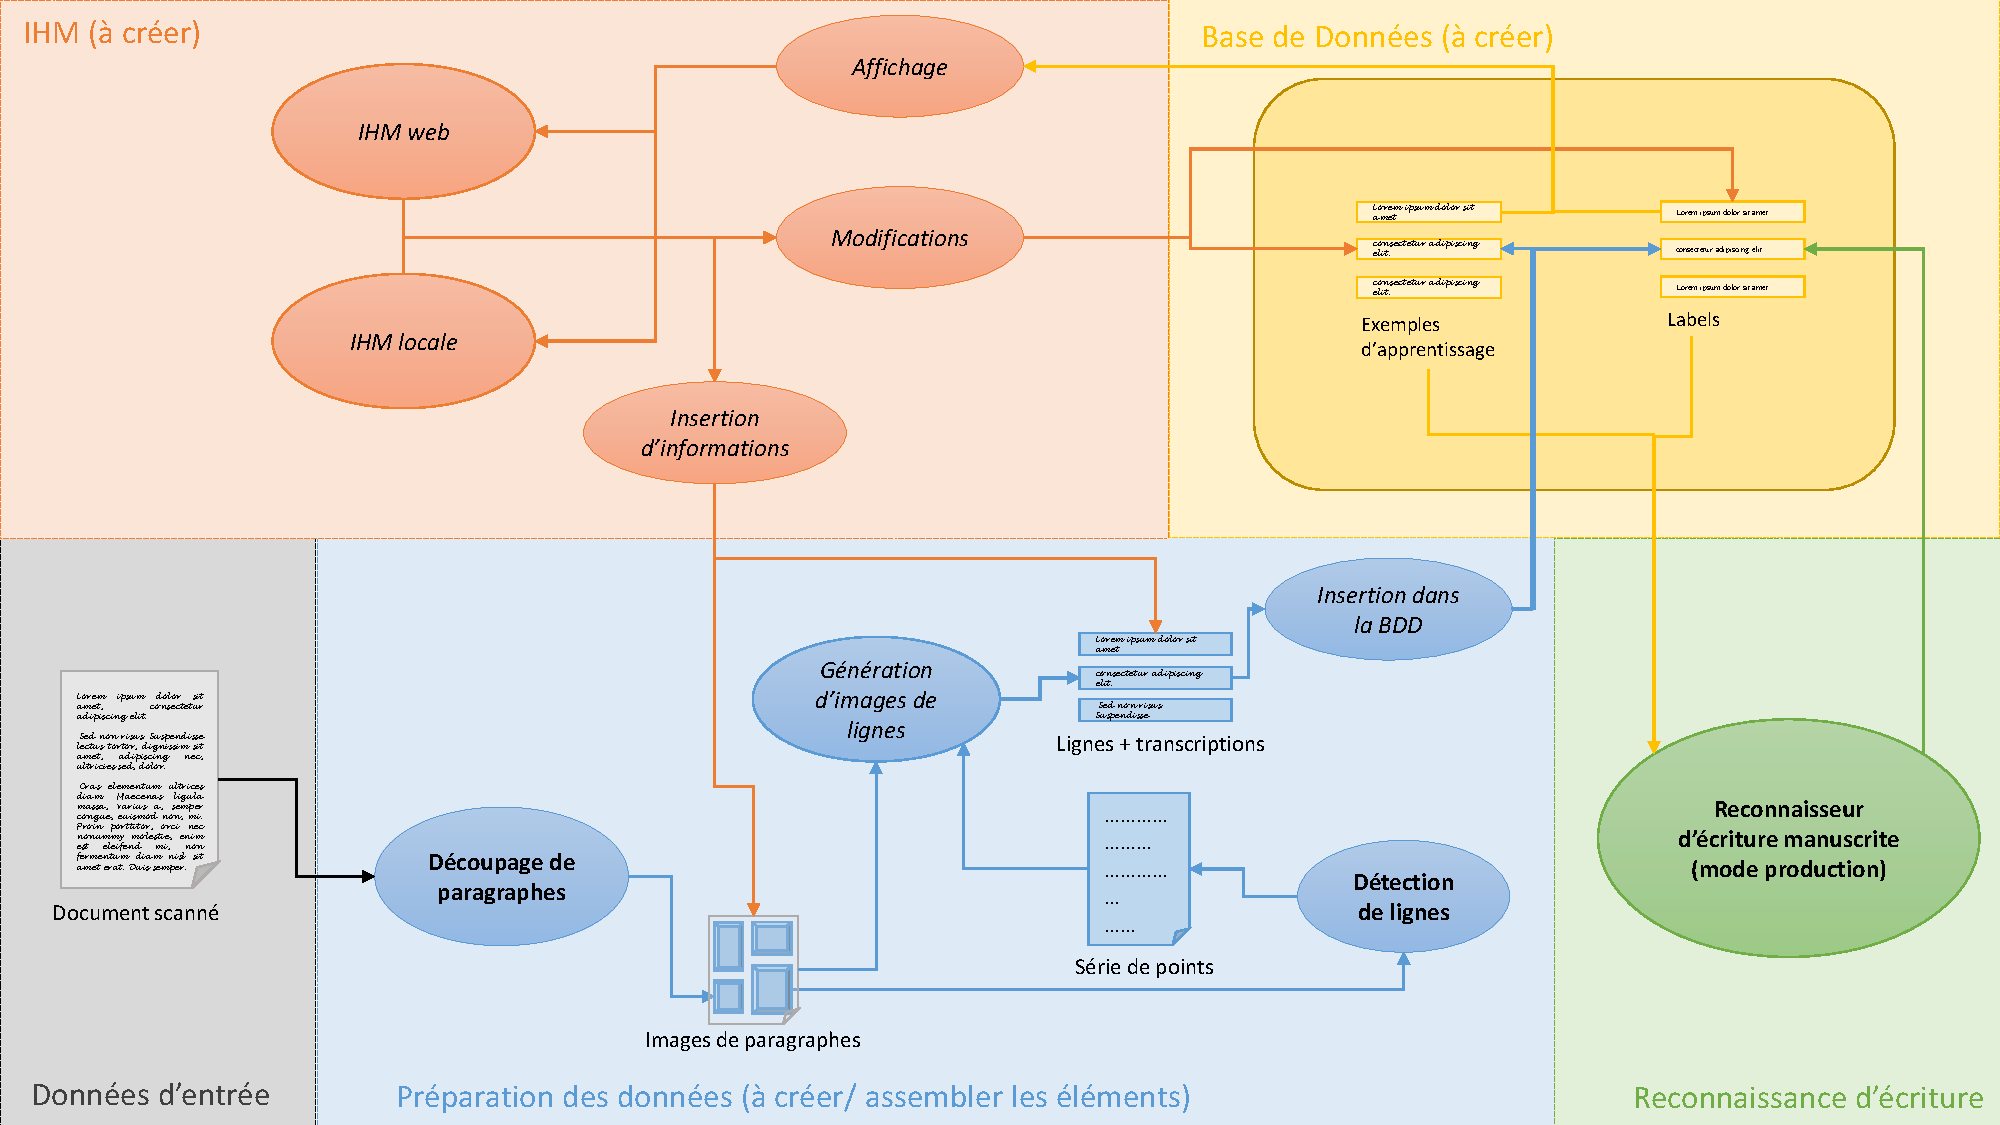
\includegraphics[width=\linewidth]{schema_mode3.1.pdf}
\end{center}
\end{mdframed}

\paragraph{}
\begin{mdframed}[frametitle={Annexe A.3.2 : Sans détection de lignes}, innerbottommargin=10]
\begin{center}
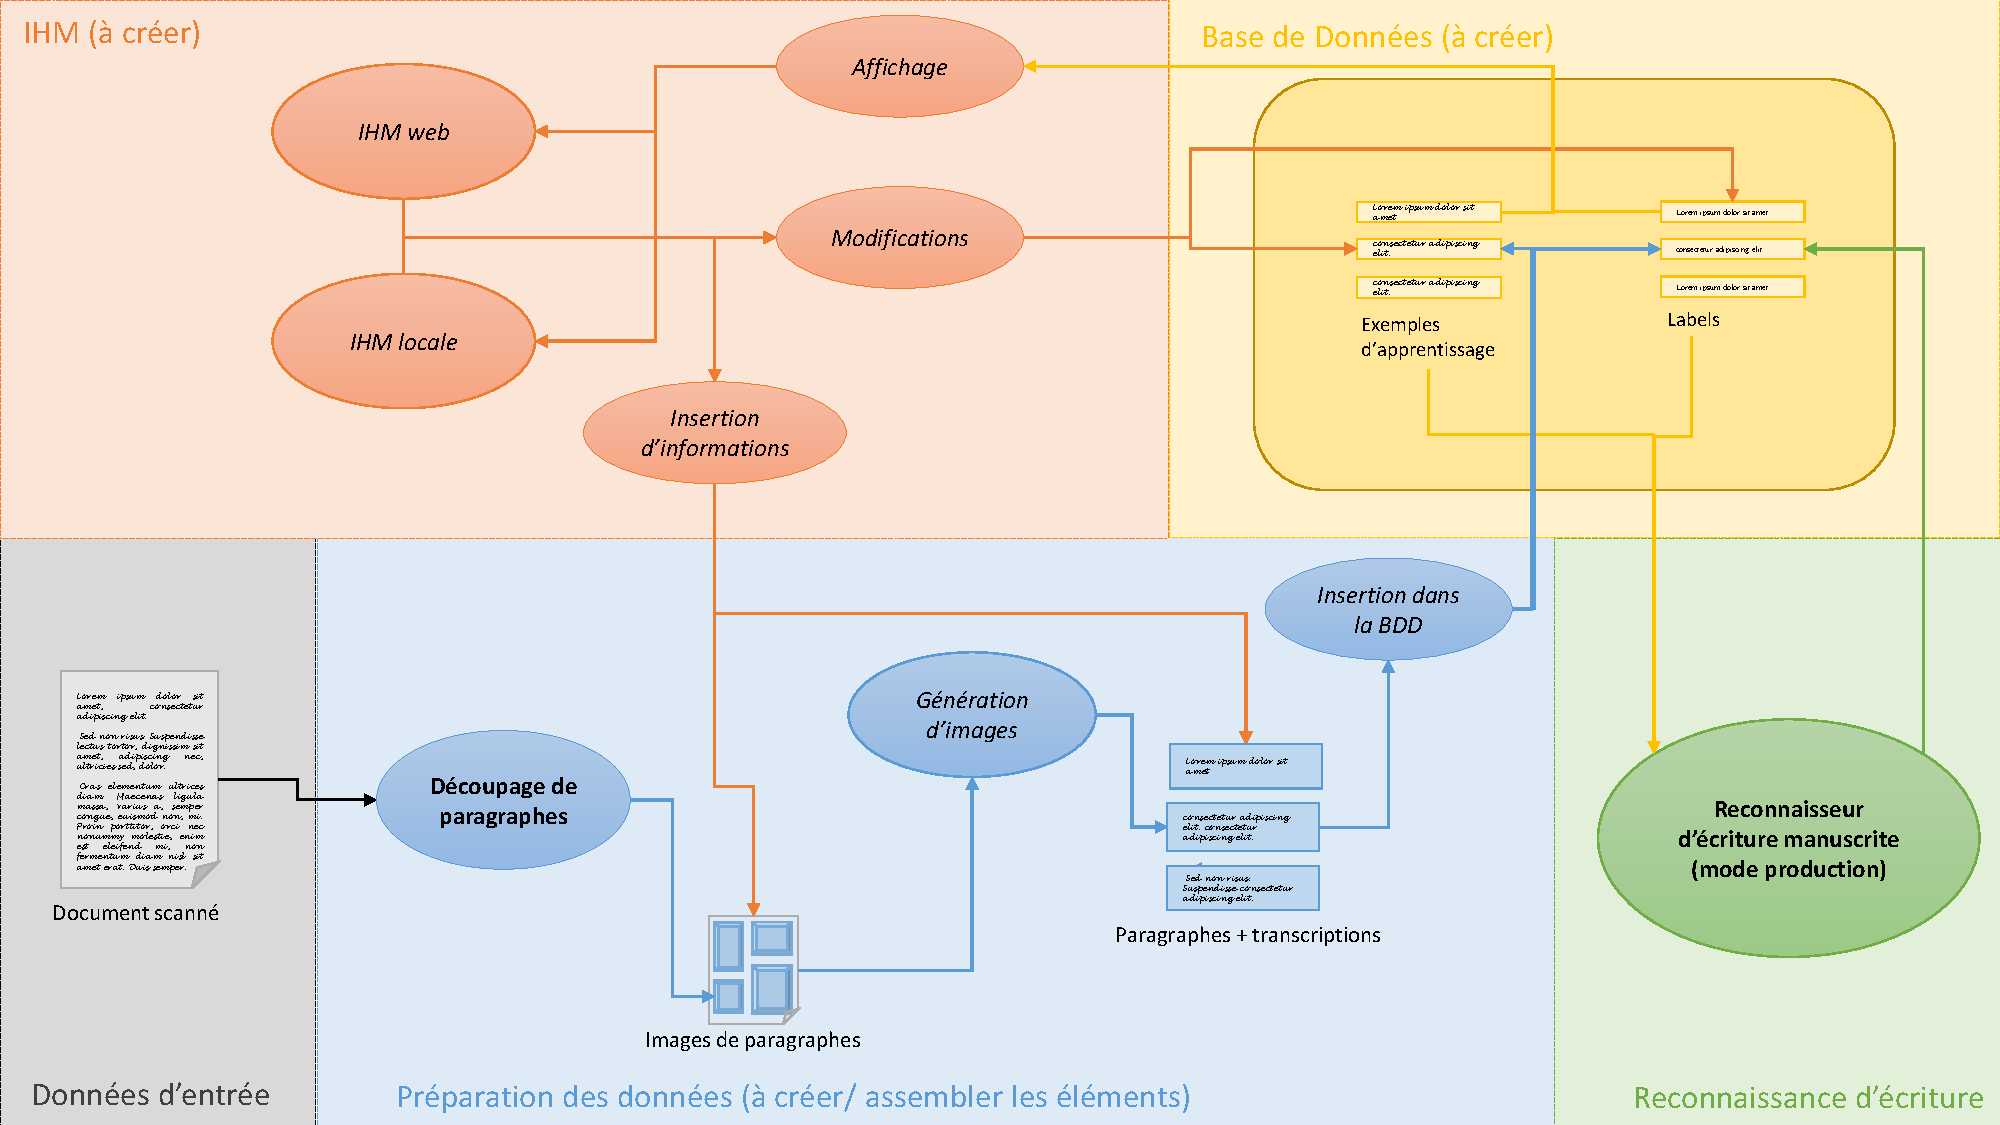
\includegraphics[width=\linewidth]{schema_mode3.2.pdf}
\end{center}
\end{mdframed}